\documentclass{article}
\usepackage[utf8]{inputenc}
\usepackage{listings}
\usepackage{xcolor}
\usepackage{appendix}
\definecolor{backcolour}{rgb}{0.95,0.95,0.92}
\definecolor{keyword}{rgb}{100,0,100}

\usepackage[acronym]{glossaries}
\usepackage{graphicx}

\makeglossaries

\newglossaryentry{function}
{
        name=function,
        description={A function is a unit of code that is often defined by its role within a greater code structure}
}

\newglossaryentry{unix}
{
        name=unix time,
        description={Also known as seconds since epoch, unix time is a system to describe a point in time. It is the number of seconds that have elapsed since 00:00:00 Thursday, 1  January 1970}
}

\newglossaryentry{mysql}
{
        name=mysql,
        description={mySQL is an open source relational database management system}
}

\newacronym{pk}{PK}{Primary Key}
\newacronym{fk}{FK}{Foreign Key}
\newacronym{sql}{SQL}{Structured Query Language}
\newacronym{php}{PHP}{Personal Home Page / Hypertext Preprocessor}
\newacronym{asc}{ASC}{Ascending}
\newacronym{desc}{DESC}{Descending}


\lstdefinestyle{mystyle}{
    basicstyle=\fontfamily{pcr}\selectfont\footnotesize,
    backgroundcolor=\color{backcolour},
    keywordstyle=\color{keyword},
    numbers=left,
    stringstyle=,
    showspaces=false,
    showstringspaces=false
}

\title{ISO Group Report}
\author{
Elliot Emmerson\\
\texttt{16120046@shrewsbury.ac.uk}\\
\texttt{e014566h@student.staffs.ac.uk}
\\  \\
Kubilay Korkmaz\\
\texttt{me@kubs.uk}\\
\texttt{15114192@shrewsbury.ac.uk}
\and
}
\date{March 2019}

\begin{document}

\maketitle

\clearpage

\tableofcontents

\clearpage

\section{Introduction}This is the documentation being used to present, and explain if necessary, the database, the data, the scripts, and the queries and their resulting outputs to achieve \textit{coursework 2} of the Information Systems in Organisations unit.

\section{Creating the Database}

Refer to appendix A

\section{Create queries to output the data in each of the six forms in the appendices}In this Task we had to create the \acrshort{sql} queries and test data to recreate the 6 appendices:

\subsection{APPENDIX 1 - A list of PFA members in alphabetical order of family name}
\subsubsection{Initial impression}To recreate this appendix it was understood that the pfa id would have to be selected, the member's first and second name, their join date, and their contributions. Also anticipated was the need to use the ``CONCAT" \gls{function} to show their full name in a single column as well as the ``ORDER BY'' and ``ASC'' keywords to order the rows appropriately.


\subsubsection{PFA Members Query}
\begin{lstlisting}[language=sql, caption=PFA Members Query, style=mystyle]
SELECT  pfa_id,
        CONCAT(carer_first_name,' ',carer_last_name)
        AS full_name,
        pfa_join_date,
        contributions
FROM    pfa 
INNER   JOIN carer 
WHERE   pfa.carer_id = carer.carer_id 
ORDER   BY carer.carer_last_name ASC
\end{lstlisting}

\subsubsection{Walk Through} Firstly, the lines 1 through 5 of \textit{Listing 1: PFA Members Query} show the columns being selected by the query. Line 1 being \textit{pfa\_id}, line 2 is the columns \textit{carer\_first\_name} and \textit{carer\_last\_name} being combined with a space in between to create the carers whole name. This is being done by using the \textbf{CONCAT} \gls{function} which joins two or more expressions together. Line 3 sets the column containing the amalgamation of \textit{carer\_first\_name} and \textit{carer\_last\_name}. Line 4 and 5 select \textit{pfa\_join\_date} and \textit{contributions} accordingly.
\\\newline
Secondly, line 6 shows the table from which the columns are being selected. This is done by using the \textbf{FROM} keyword followed by the table name, which in this case, is \textit{pfa}.
\\\newline
Thirdly, line 7 is where the table \textit{pfa} is joined with \textit{carer}. This is done so it's possible to get the columns from the \textit{carer} table in the query. The table is joined by first using the keyword that defines the type of join to be carried out, in this case an inner join is required. To do this the \textbf{INNER} keyword is used followed by the \textbf{JOIN} keyword to initiate the join. Then the table name to be joined is written in this case \textit{carer}.
\\\newline
Next, line 8 is the join condition as denoted by the \textbf{WHERE} keyword. This line uses the \acrfull{pk} and \acrfull{fk} to join tables which have a relationship. In this example it shows that the tables will be joined when foreign key \textit{pfa.carer\_id} equals the primary key \textit{carer.carer\_id}.
\\\newline
Finally, line 9 defines the order of which the rows are listed. The keyword \textbf{ORDER BY} followed by the column name \textit{carer.carer\_last\_name} shows that the results will be ordered using the  \textit{carer\_last\_name} column from the \textit{carer} table. The \textbf{\acrshort{asc}} keyword that follows defines the way that the rows are ordered. In this case \textbf{``\acrshort{asc}''} refers to an ascending order as the appendix required.

\subsubsection{Query Results}
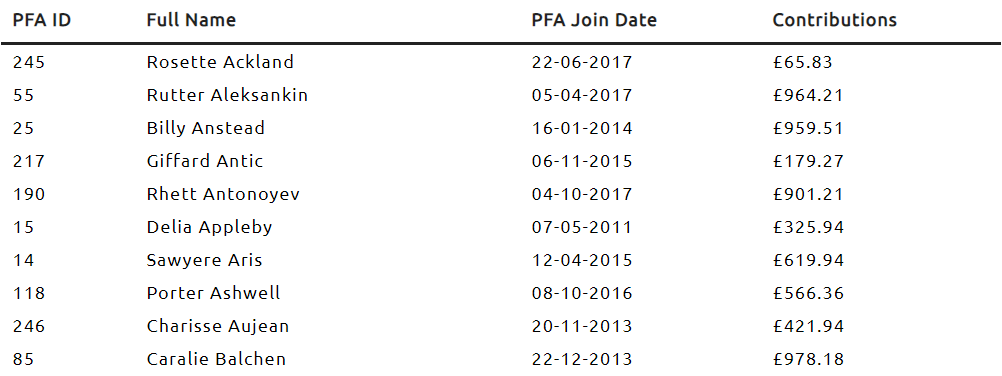
\includegraphics[width=\linewidth]{images/01.png}

\subsection{APPENDIX 2 A list of staff with managers}
\subsubsection{Initial Impression} On first look this appendix doesn't look to introduce anything new and is just a variation on the previous appendix by selecting more rows from more tables.

\subsubsection{All Staff Members Query}
\begin{lstlisting}[language=sql, caption=All Staff Members Query, style=mystyle]
SELECT  staff_id,
        CONCAT(staff_first_name,' ',staff_last_name) 
        AS staff_full_name,
        role_name,
        staff_date_hired,
        staff_hourly_salary,
        staff.line_manager_id,
        CONCAT(line_manager_first_name,' ',line_manager_last_name) 
        AS line_manager_full_name 
FROM  ((staff   INNER JOIN role ON role.role_id = staff.role_id)
                INNER JOIN line_manager ON staff.line_manager_id 
                = line_manager.line_manager_id)
ORDER   BY staff_date_hired DESC
\end{lstlisting}

\subsubsection{Walk Through} Similar to the previous appendix lines 1 through 9 outline the rows selected. Different to the previous appendix though is where the tables are joined. Instead of a single join of two tables this is a double join combining 3 tables. On line 10 the tables \textit{role} and \textit{staff} are joined through the \acrshort{pk} and \acrshort{fk}  (\textit{role.role\_id} and \textit{staff.role\_id}). On the next line, line 11, the tables \textit{line\_manager} and \textit{staff} are joined through the \acrshort{pk} and \acrshort{fk} (\textit{line\_manager.line\_manager\_id} and \textit{staff.line\_manager\_id}).

\subsubsection{Query Results}
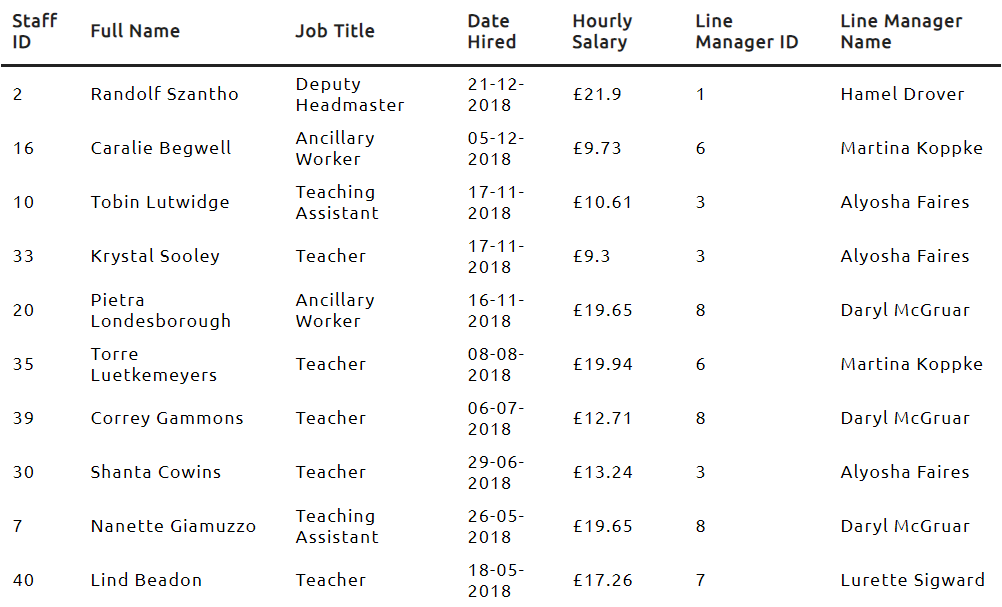
\includegraphics[width=\linewidth]{images/02.png}

\subsection{APPENDIX 3 Resource hire sheet}
\subsubsection{Initial Impression} At first look at this appendix it would appear to be very similar only with a slightly different appearance to the output visually. The top part of the appendix shows the entries for each column of a single row, whilst it wasn't abundantly clear it was agreed upon in the group that this must be for inserting data for booking a resource.

\subsubsection{Resource Hire Sheet SELECT Query}
\begin{lstlisting}[language=sql, caption=Resource Hire Sheet SELECT Query, style=mystyle]
SELECT  resource_booking_id, 
        resource_booking.resource_id, 
        resource_name, 
        resource_booking.staff_id, 
        CONCAT(staff_first_name, ' ', staff_last_name) 
        AS staff_full_name, 
        date_out, 
        number_of_days 
FROM  ((resources
        INNER JOIN resource_booking 
        ON resource_booking.resource_id = resources.resource_id)
        INNER JOIN staff
        ON resource_booking.staff_id = staff.staff_id)
ORDER   BY date_out DESC
\end{lstlisting}

\newpage

\subsubsection{Walk Through} The query structure for this appendix is essentially the same as the previous appendix so there is nothing to go into detail on other than the use of \acrfull{desc} instead of \acrfull{asc}.
\subsubsection{Query Results}
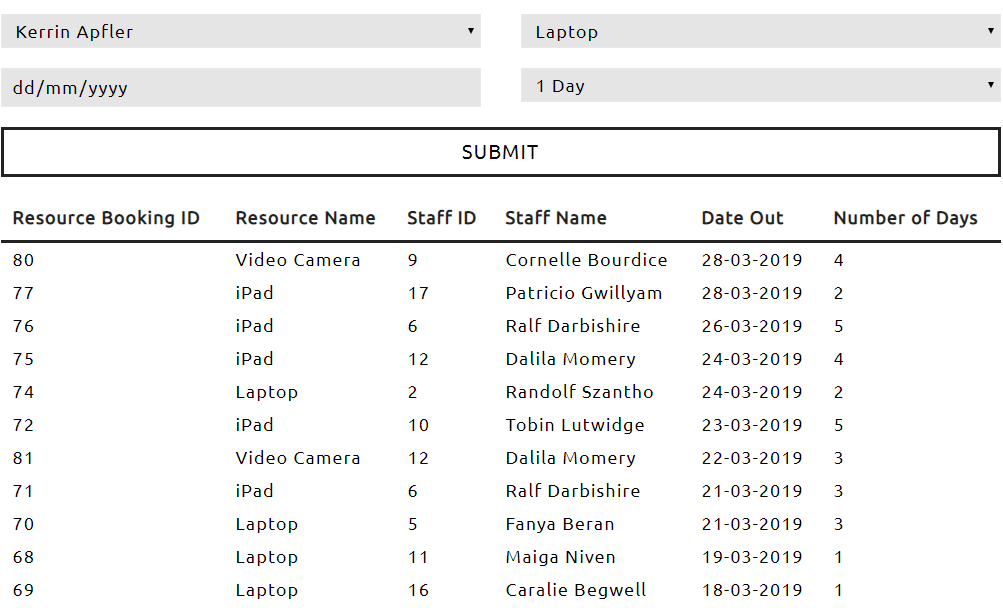
\includegraphics[width=\linewidth]{images/03.png}

\subsubsection{Hire Resource INSERT Query}
\begin{lstlisting}[language=sql, caption=Hire Resource INSERT Query, style=mystyle]
INSERT  INTO 
        resource_booking(
        resource_id, 
        staff_id, 
        date_out, 
        number_of_days) 
VALUES  (?, ?, ?, ?)
\end{lstlisting}

\subsubsection{Walk Through} In this query a row is inserted into the \textit{resource\_booking} table. On line 1 the keywords \textbf{INSERT} and \textbf{INTO} initiate the process of inserting the row. The 2nd line denotes which table to insert the row into, in this case the \textit{resource\_booking} table. Lines 3 to 6 shows which rows to insert data into. The last line uses the \textbf{VALUES} keyword to. The \textit{question marks} show where the data will be inserted via \acrshort{php}.

\subsection{APPENDIX 4 Faculty teacher listing}
\subsubsection{Initial Impression} At first glance, the query described in the appendix looks like it will require a large amount of joins to extract all data that is necessary, however there are no complex \textbf{ORDER BY} or \textbf{LIMIT} keywords that are necessary to successfully create the query.

\subsubsection{Faculty Teacher Listing Query}
\begin{lstlisting}[language=sql, caption=Faculty Teacher Listing Query, style=mystyle]
SELECT  faculty.faculty_id, 
        subject_link.subject_id, 
        subject.subject_name, 
        staff.staff_id, 
        CONCAT(staff_first_name, ' ', staff_last_name) 
        AS full_name, 
        faculty.faculty_name 
FROM    subject_link
INNER   JOIN staff ON staff.STAFF_ID = subject_link.staff_id
INNER   JOIN subject ON subject.SUBJECT_ID = subject_link.subject_id
INNER   JOIN faculty ON faculty.faculty_id = subject.faculty_id
\end{lstlisting}

\subsubsection{Walk Through} Firstly, all the parameters must be selected accordingly (due to the fact that multiple tables are being used, an \textit{*} symbol can not be used). The query requires a lot of table joins, as there is a large amount of data required in the \textbf{SELECT} portion of the query.
\\\newline
Secondly, the data originally becomes extracted from the table \textit{subject\_link}, as it allows the \textit{subject\_id}, \textit{staff\_id} and \textit{faculty\_id} to be joined instantly. With the three id's that have been extracted from the \textit{subject\_link} table, further tables named \textit{staff}, \textit{faculty} and \textit{subject} to extract additional data.
\\\newline
As all of the tables have been joined, the extra data such as \textit{staff\_name}, \textit{faculty\_name} and \textit{subject\_name} can be selected successfully.

\subsubsection{Query Results}
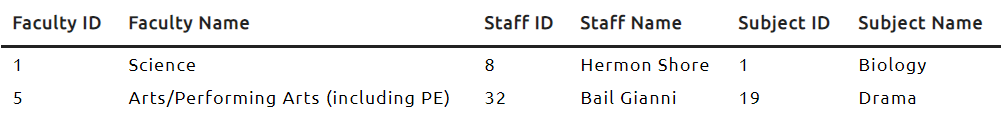
\includegraphics[width=\linewidth]{images/04.png}


\subsection{APPENDIX 5 Faculty member listing}
\subsubsection{Initial Impression} The initial impressions of this appendix were that the tables \textit{staff} with \textit{faculty} would need to be linked using the link table \textit{faculty\_link}.

\subsubsection{Faculty Member Listing Query}
\begin{lstlisting}[language=sql, caption=Faculty Member Listing Query, style=mystyle]
SELECT  faculty.faculty_id, 
        faculty.faculty_name, 
        staff.staff_id, 
        CONCAT(staff_first_name, ' ', staff_last_name) 
        AS full_name, 
        faculty_link.date_joined 
FROM    faculty_link
INNER   JOIN staff ON staff.staff_id = faculty_link.staff_id
INNER   JOIN faculty ON faculty.faculty_id = faculty_link.faculty_id
\end{lstlisting}

\subsubsection{Walk through} As was done in the previous queries the lines 1 through 6 are the columns being selected by using the \textbf{SELECT} keyword. Line 7 is the table to query, with 8 and 9 joining 2 extra tables being linked through their \textit{\acrshort{pk}} and \textit{\acrshort{fk}} relationship.

\subsubsection{Query Results}
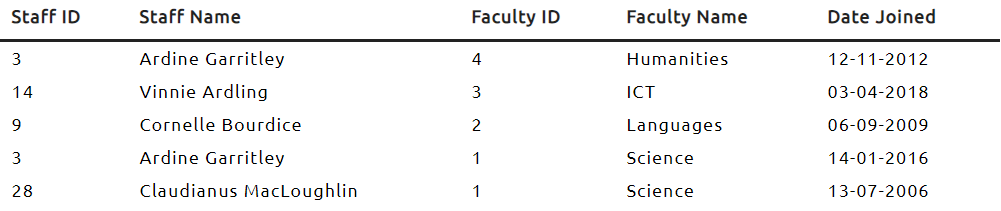
\includegraphics[width=\linewidth]{images/05.png}

\subsection{APPENDIX 6 Room request sheet}
\subsubsection{Initial Impression} As this appendix displays a form that will allow the user to book a room, it was known from early on that there would be multiple queries necessary. In the demo, the form contained data that would need to be inserted into the database using an \textbf{INSERT INTO} keyword, and the data can be extracted and displayed using simple \textbf{SELECT} and \textbf{JOIN} keywords.

\subsubsection{Room Booking INSERT Query}
\begin{lstlisting}[language=sql, caption=Room Booking Insert, style=mystyle]
INSERT  INTO 
        room_booking(
        staff_id, 
        room_id, 
        booking_date, 
        duration)
VALUES  (?, ?, ?, ?)
\end{lstlisting}

\subsubsection{Walk through} Firstly, the query that handles booking uses an \textbf{INSERT INTO} keyword to enter data into the \textit{room\_booking} table. The values are taken from a \acrshort{php} script used in the demo. The user will enter the \textit{staff\_id}, \textit{room\_id}, \textit{booking\_date} and the \textit{duration} of the booking.

\subsubsection{Room Booking SELECT Query}
\begin{lstlisting}[language=sql, caption=Room Booking Sheet, style=mystyle]
SELECT  room_booking_id, 
        room_booking.room_id, 
        room_name, 
        room_booking.staff_id, 
        CONCAT(staff_first_name, ' ', staff_last_name) 
        AS staff_full_name, 
        booking_date, 
        duration 
FROM  ((room
INNER   JOIN room_booking ON room_booking.room_id = room.room_id)
INNER   JOIN staff ON room_booking.staff_id = staff.staff_id)
ORDER   BY duration DESC
\end{lstlisting}

\subsubsection{Walk through} To extract all the data from the \textit{room\_booking} table, two other tables had to be joined (\textit{staff}, \textit{room}) so that staff and room details could be extracted and selected in the query. The data was then ordered by \acrfull{desc} using \textit{ORDER BY}.

\subsubsection{Query Results}
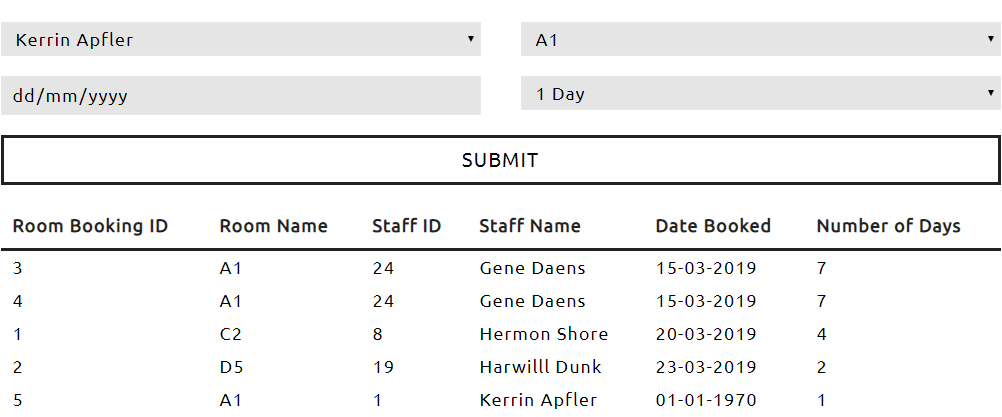
\includegraphics[width=\linewidth]{images/06.png}

\newpage

\section{Create queries to show each of the following}

\subsection{Teachers who are also parents}
\subsubsection{Initial Impression} This query really took a lot of thinking and theorising, the ability to relate staff to parents and students without duplicating data was not factored into the original plan, therefore the database had to be modified a slight bit.
\\\newline
A new table named \textit{family} had to be created, link tables had to also be created so that students, staff and parents could be linked together. This also solved a dilemma of being able to have 2 students relating to one parent.

\subsubsection{Teachers Who Are Also Parents Query}
\begin{lstlisting}[language=sql, caption=Teachers Who Are Also Parents Query, style=mystyle]
SELECT  staff_family_link.family_id, 
        staff_family_link.staff_id, 
        CONCAT(staff_first_name, ' ', staff_last_name)
        AS staff_name, 
        COUNT(student_family_link.family_id) 
        AS number_of_students 
FROM    staff
INNER   JOIN staff_family_link 
        ON staff_family_link.staff_id = staff.staff_id
INNER   JOIN family 
        ON family.family_id = staff_family_link.family_id
INNER   JOIN student_family_link 
        ON student_family_link.family_id = staff_family_link.family_id
GROUP   BY staff_family_link.family_id
\end{lstlisting} 

\subsubsection{Walk Through} Firstly, the parameters \textit{family\_id}, \textit{staff\_id}, \textit{staff\_name} (by using the 'CONCAT()' \gls{function}) and \textit{number\_of\_students} (by using the 'COUNT()' \gls{function}).
\\\newline
The original table that the data is extracted from is the \textit{staff} table, and the other tables \textit{staff\_family\_link}, \textit{family} and \textit{student\_family\_link} are required to further link necessary tables in order to extract all data needed. So the \textbf{INNER JOIN} keyword is used to join these tables adequately.
\\\newline
Finally, after all the tables are joined at the specific points, the whole table must be grouped by \textit{staff\_family\_link.family\_id}, as it will ensure to group the whole dataset by the specific column stated.

\subsubsection{Query Results}
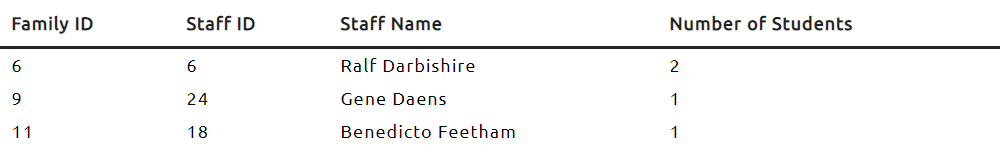
\includegraphics[width=\linewidth]{images/07.png}

\subsection{The resources that have been hired less than 3 times}
\subsubsection{Initial Impression} At first look, this query seemed as it would need the use of the \textbf{COUNT()} function, as it would need to access the amount of times each \textit{resource\_id} has been used in the \textit{resource\_booking} table, and show details such as \textit{resource\_name} based on the results of \textit{resource\_booking}. 

\subsubsection{The resources that have been hired less than 3 times Query}
\begin{lstlisting}[language=sql, caption=The resources that have been hired less than 3 times Query, style=mystyle]
SELECT  resources.resource_id, 
        resources.resource_name, 
        COUNT(resource_booking.resource_id) 
        AS times_hired 
FROM    resources
INNER   JOIN resource_booking 
        ON resource_booking.resource_id = resources.resource_id
GROUP   BY resource_booking.resource_id 
        HAVING COUNT(resource_booking.resource_id) < 3
ORDER   BY COUNT(resource_booking.resource_id) DESC
\end{lstlisting} 

\subsubsection{Walk Through} First, \textit{resource\_id}, \textit{resource\_name} and \textit{times\_hired} (calculated from the \textbf{COUNT()} function) must be selected originally from the \textit{resources} table.
\\\newline
Secondly, an \textbf{INNER JOIN} keyword is used to link the \textit{resource\_booking} table based on the column \textit{resource\_id}. Furthermore, the \textbf{GROUP BY} keyword is used to group all the data selected by the \textit{resource\_id} column where the \textbf{COUNT()} result of \textit{resource\_id} is less than three. Finally, the data is ordered by the \textbf{COUNT()} result of \textit{resource\_id} \acrshort{desc} using the \textbf{ORDER BY} keyword for convenience.

\subsubsection{Query Results}
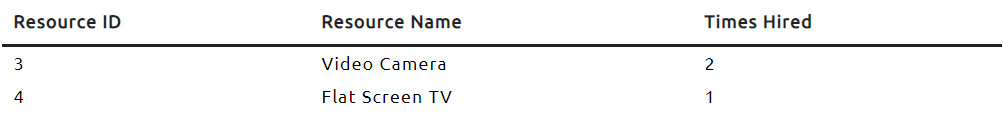
\includegraphics[width=\linewidth]{images/08.png}

\newpage

\subsection{The staff who have worked for all the departments}
\subsubsection{Initial Impression} On first impression this task appeared to be trivial in it's difficulty. All was needed was staff that had 4 different departments in the \textit{department\_link} table. And whilst yes you are able to return the number of unique departments a staff member has worked in using functions like \textbf{COUNT} to display the number of rows and \textbf{DISTINCT} to only select the ones that were distinct or different. The initial query used to attempt this task, seen below, return an error.

\begin{lstlisting}[language=sql, caption=The staff who have worked for all the departments Query First Attempt, style=mystyle]
SELECT  department_link.staff_id,
        CONCAT(staff_first_name, ' ', staff_last_name) 
        AS staff_name, 
        COUNT(DISTINCT department_id) 
        AS number_of_departments 
FROM    department_link
INNER   JOIN staff 
        ON staff.staff_id = department_link.staff_id
WHERE   COUNT(DISTINCT department_id) = 4
GROUP   BY department_link.staff_id
\end{lstlisting} 
The error returned was \textit{`\#1111 - Invalid use of group function'}.
\\\\
Upon further research it became apparent that use of \textit{aggregate} or \textit{group} functions was impossible in a \textbf{WHERE} clause. \textbf{COUNT} being a aggregate function, the root of the error had be found. This is when line 9, the \textbf{WHERE} clause, of the first query was removed and replaced with a \textbf{HAVING} clause. This allowed the use of the \textbf{COUNT} function with a comparison operator such as `='.

\subsubsection{The staff who have worked for all the departments Query}
\begin{lstlisting}[language=sql, caption=The staff who have worked for all the departments Query, style=mystyle]
SELECT  department_link.staff_id,
        CONCAT(staff_first_name, ' ', staff_last_name) 
        AS staff_name, 
        COUNT(DISTINCT department_id) 
        AS number_of_departments 
FROM    department_link
INNER   JOIN staff 
        ON staff.staff_id = department_link.staff_id
GROUP   BY department_link.staff_id
HAVING  COUNT(DISTINCT department_id) = 
       (SELECT COUNT(DISTINCT department_id) FROM department)
\end{lstlisting} 

\subsubsection{Walk Through} On lines 1 through 5 the columns are being selected. Line 6 is the table to query with lines 7 and 8 joining the \textit{department\_link} table with the \textit{staff} table using the \acrshort{pk} and \acrshort{fk}, \textit{staff.staff\_id} and \textit{department\_link.staff\_id}.
\\\newline
Line 9 groups the rows by \textit{department\_link.staff\_id} and then line 10 filters the results using the \textbf{HAVING} keyword. The results are then filtered by the \textbf{COUNT} of unique departments that are equal to  the number of total departments. This would not have been possible if a \textbf{WHERE} clause was used.
\\\newline
The final line, line 11, is a sub query to return the \textbf{COUNT} of departments to use in the comparison on the previous line. If the integer 4, which is the current number of departments at the time of writing, had been used instead it would require rewriting the query every time a new deparment was added.

\subsubsection{Query Results}
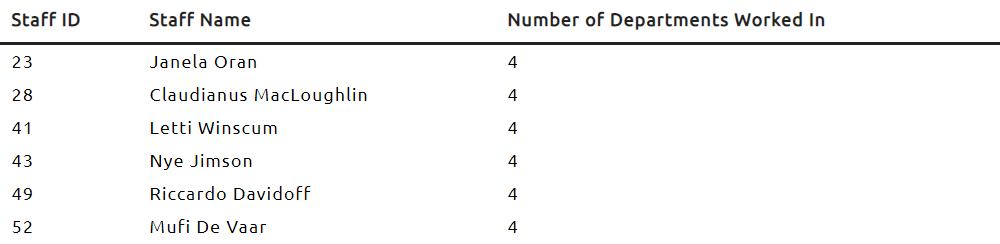
\includegraphics[width=\linewidth]{images/09.png}

\subsection{The details of the teachers, whose surname starts with the same letter as the person who has attended the most meetings}
\subsubsection{Initial Impression} An initial look at this query resulted in a long planning stage to help formulate the query. After first trying to instantly write it, the realisation that writing out my thoughts would be the best idea to solve the problem. It was clear that the \textbf{SUBSTRING()} function would be necessary as the first letter of the \textit{staff\_last\_name} column must be saved, and used later on in the query in a clause to get data from the \textit{staff} table.


\subsubsection{The details of the teachers, whose surname starts with the same letter as the person who has attended the most meetings Query}
\begin{lstlisting}[language=sql, caption=The details of the teachers whose surname starts with the same letter as the person who has attended the most meetings, style=mystyle]
SELECT  staff_id,
        CONCAT(staff_first_name, ' ', staff_last_name) AS staff_name,
        staff_date_hired,
        staff_hourly_salary,
        staff_address,
        staff_phone_number
FROM    staff
WHERE   SUBSTRING(staff_last_name, 1, 1) =
       (SELECT SUBSTRING(staff_last_name, 1, 1)
FROM    meeting_attendee
INNER   JOIN staff ON staff.staff_id = meeting_attendee.staff_id
GROUP   BY meeting_attendee.staff_id
ORDER   BY COUNT(meeting_attendee.staff_id) DESC
LIMIT   1)
\end{lstlisting} 
\subsubsection{Walk Through} To begin, the specified data: \textit{staff\_id}, \textit{staff\_name}, \textit{staff\_date\_hired}, \textit{staff\_address} and \textit{staff\_phone\_number} was selected originally from the \textit{staff} table.
\\\newline
A \textbf{WHERE} clause is then used to get data only from rows where the \textbf{SUBSTRING(val, 1, 1)} result of \textit{staff\_last\_name} (the first letter) was equal to the output of a new \textbf{SELECT} statement.
\\\newline
The new \textbf{SELECT} statement consisted of selecting the first letter of the \textit{staff\_last\_name} that has attended the most meetings (as found in the \textit{meeting\_attendee} table. This is then finalised by using the \textbf{LIMIT} keywords to limit the result output to just 1 row.

\subsubsection{Query Results}
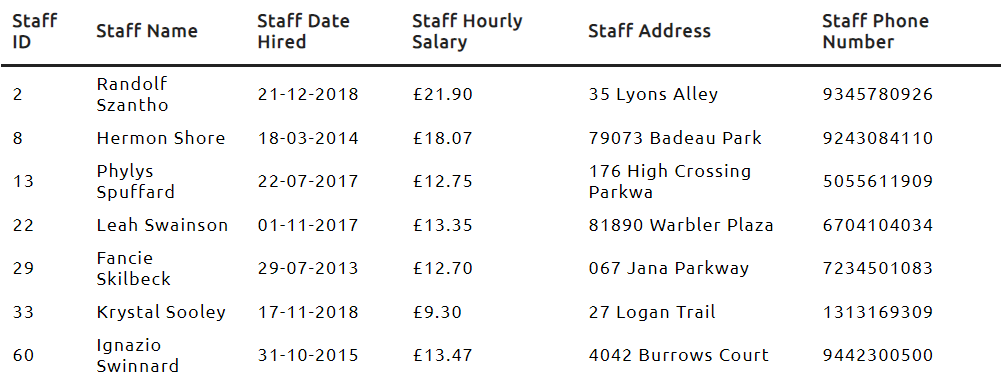
\includegraphics[width=\linewidth]{images/10.png}

\section{Create queries to alter the database in the following ways}

\subsection{Alter the employee table to include a numeric column called "payscale" query}
\begin{lstlisting}[language=sql, caption=Add Payscale, style=mystyle]
ALTER   TABLE staff ADD payscale double(11,2)
\end{lstlisting}

\subsubsection{Walk Through} The \textbf{ALTER TABLE} keyword is used to alter the pre-existing table called \textit{staff}, and the \textbf{ADD} keyword allows a column to be added to the table. For this specific entry, a double was used as payment commonly uses decimal places. So the two parameters parsed in the brackets after double are: (length, decimal places). 11 is a given as it is a 32 bit number and the 2 used in the decimal place parameter is set as money used 2 decimal places.

\subsection{Insert the value of 1 into the field for all employees}
\begin{lstlisting}[language=sql, caption=Insert Value, style=mystyle]
UPDATE  staff
SET     payscale = 1;
\end{lstlisting}

\subsubsection{Walk Through} This simple query uses the \textbf{UPDATE} keyword to update rows in the specified table \textit{staff}, the \textbf{SET} keyword allows the data in a specific column to be set to anything in the datatype's possibility. For this example, the column \textit{payscale} was set to 1 for all users.

\subsection{Update the payscale value for employees who have been working at the school for over five years to the value of 2}
\begin{lstlisting}[language=sql, caption=Update Payscale, style=mystyle]
UPDATE  staff
SET     payscale = 2
WHERE   staff_date_hired < UNIX_TIMESTAMP(NOW() - INTERVAL 5 YEAR);
\end{lstlisting}

\subsubsection{Walk Through} For this query, the same \textbf{UPDATE} and \textbf{SET} keywords were used as in the previous query, however this time a \textbf{WHERE} clause was used to only change details for specific rows.
\\\newline
In order to understand which rows contained a staff member that has been working for the school for more than 5 years, the \textit{less than (<)} operator is used to work out the difference between \gls{unix} now, and the \gls{unix} time stored in \textit{staff\_date\_hired}. If the number is equal to 5 years in \gls{unix} time, the data will be updated in that row.

\subsection{Delete resources that have never been hired}
\begin{lstlisting}[language=sql, caption=Delete Resources, style=mystyle]
DELETE  FROM resources
WHERE   resource_id 
NOT IN (SELECT resource_booking.resource_id 
        FROM resource_booking)
\end{lstlisting}

\subsubsection{Walk Through} Firstly, the \textbf{DELETE} keyword was used to delete all rows depicted in the latter part of the query from the \textit{resources} table. A \textbf{WHERE} clause is used to split up data where the value of \textit{resource\_id} is \textbf{NOT IN} the following query. The query gets rows from the \textit{resource\_booking} table by selecting \textit{resource\_id} from the \textit{resource\_booking} table.

\newpage

\section{Appendicies}
\appendix

\section{Database Creation}
\begin{lstlisting}[language=sql, caption=Database Generation Script, style=mystyle]

SET SQL_MODE = "NO_AUTO_VALUE_ON_ZERO";
SET time_zone = "+00:00";

--
-- Database: `hopeville_school`
--
CREATE  DATABASE IF NOT EXISTS `hopeville_school` 
DEFAULT CHARACTER SET latin1 COLLATE latin1_swedish_ci;
USE `hopeville_school`;

-- --------------------------------------------------------

--
-- Table structure for table `carer`
--

CREATE TABLE `carer` (
  `carer_id` int(11) NOT NULL,
  `carer_first_name` varchar(64) NOT NULL,
  `carer_last_name` varchar(64) NOT NULL,
  `carer_address` varchar(128) NOT NULL,
  `carer_postcode` varchar(16) DEFAULT NULL,
  `carer_phone_number` varchar(32) NOT NULL
) ENGINE=InnoDB DEFAULT CHARSET=latin1;

-- --------------------------------------------------------

--
-- Table structure for table `carer_family_link`
--

CREATE TABLE `carer_family_link` (
  `carer_family_link_id` int(11) NOT NULL,
  `family_id` int(11) NOT NULL,
  `carer_id` int(11) NOT NULL
) ENGINE=InnoDB DEFAULT CHARSET=latin1;

-- --------------------------------------------------------

--
-- Table structure for table `department`
--

CREATE TABLE `department` (
  `department_id` int(11) NOT NULL,
  `department_name` varchar(64) NOT NULL,
  `department_age_group` varchar(16) NOT NULL
) ENGINE=InnoDB DEFAULT CHARSET=latin1;

-- --------------------------------------------------------

--
-- Table structure for table `department_link`
--

CREATE TABLE `department_link` (
  `department_link_id` int(11) NOT NULL,
  `department_id` int(11) NOT NULL,
  `staff_id` int(11) NOT NULL,
  `start_date` int(11) NOT NULL,
  `end_date` int(11) NOT NULL
) ENGINE=InnoDB DEFAULT CHARSET=latin1;

-- --------------------------------------------------------

--
-- Table structure for table `faculty`
--

CREATE TABLE `faculty` (
  `faculty_id` int(11) NOT NULL,
  `faculty_name` varchar(64) NOT NULL
) ENGINE=InnoDB DEFAULT CHARSET=latin1;

-- --------------------------------------------------------

--
-- Table structure for table `faculty_link`
--

CREATE TABLE `faculty_link` (
  `faculty_link_id` int(11) NOT NULL,
  `staff_id` int(11) NOT NULL,
  `faculty_id` int(11) NOT NULL,
  `date_joined` int(11) NOT NULL
) ENGINE=InnoDB DEFAULT CHARSET=latin1;

-- --------------------------------------------------------

--
-- Table structure for table `family`
--

CREATE TABLE `family` (
  `family_id` int(11) NOT NULL
) ENGINE=InnoDB DEFAULT CHARSET=latin1;

-- --------------------------------------------------------

--
-- Table structure for table `line_manager`
--

CREATE TABLE `line_manager` (
  `line_manager_id` int(11) NOT NULL,
  `line_manager_first_name` varchar(64) NOT NULL,
  `line_manager_last_name` varchar(64) NOT NULL,
  `line_manager_date_hired` int(11) NOT NULL,
  `line_manager_hourly_salary` double(11,2) NOT NULL,
  `line_manager_address` varchar(128) NOT NULL,
  `line_manager_postcode` varchar(32) DEFAULT NULL,
  `line_manager_phone_number` varchar(32) NOT NULL
) ENGINE=InnoDB DEFAULT CHARSET=latin1;

-- --------------------------------------------------------

--
-- Table structure for table `meeting`
--

CREATE TABLE `meeting` (
  `meeting_id` int(11) NOT NULL,
  `meeting_start_time` int(11) NOT NULL,
  `meeting_duration` int(11) NOT NULL
) ENGINE=InnoDB DEFAULT CHARSET=latin1;

-- --------------------------------------------------------

--
-- Table structure for table `meeting_attendee`
--

CREATE TABLE `meeting_attendee` (
  `meeting_attendee_id` int(11) NOT NULL,
  `meeting_id` int(11) NOT NULL,
  `staff_id` int(11) NOT NULL
) ENGINE=InnoDB DEFAULT CHARSET=latin1;

-- --------------------------------------------------------

--
-- Table structure for table `pfa`
--

CREATE TABLE `pfa` (
  `pfa_id` int(11) NOT NULL,
  `carer_id` int(11) NOT NULL,
  `pfa_join_date` int(11) NOT NULL,
  `contributions` double(11,2) NOT NULL
) ENGINE=InnoDB DEFAULT CHARSET=latin1;

-- --------------------------------------------------------

--
-- Table structure for table `resources`
--

CREATE TABLE `resources` (
  `resource_id` int(11) NOT NULL,
  `resource_name` varchar(64) NOT NULL,
  `resource_amount` int(11) NOT NULL
) ENGINE=InnoDB DEFAULT CHARSET=latin1;

-- --------------------------------------------------------

--
-- Table structure for table `resource_booking`
--

CREATE TABLE `resource_booking` (
  `resource_booking_id` int(11) NOT NULL,
  `resource_id` int(11) NOT NULL,
  `staff_id` int(11) NOT NULL,
  `date_out` int(11) NOT NULL,
  `number_of_days` int(11) NOT NULL
) ENGINE=InnoDB DEFAULT CHARSET=latin1;

-- --------------------------------------------------------

--
-- Table structure for table `role`
--

CREATE TABLE `role` (
  `role_id` int(11) NOT NULL,
  `role_name` varchar(64) NOT NULL
) ENGINE=InnoDB DEFAULT CHARSET=latin1;

-- --------------------------------------------------------

--
-- Table structure for table `room`
--

CREATE TABLE `room` (
  `room_id` int(11) NOT NULL,
  `room_name` varchar(32) NOT NULL
) ENGINE=InnoDB DEFAULT CHARSET=latin1;

-- --------------------------------------------------------

--
-- Table structure for table `room_booking`
--

CREATE TABLE `room_booking` (
  `room_booking_id` int(11) NOT NULL,
  `staff_id` int(11) NOT NULL,
  `room_id` int(11) NOT NULL,
  `booking_date` int(11) NOT NULL,
  `duration` int(11) NOT NULL
) ENGINE=InnoDB DEFAULT CHARSET=latin1;

-- --------------------------------------------------------

--
-- Table structure for table `staff`
--

CREATE TABLE `staff` (
  `staff_id` int(11) NOT NULL,
  `staff_first_name` varchar(64) NOT NULL,
  `staff_last_name` varchar(64) NOT NULL,
  `role_id` int(11) NOT NULL,
  `staff_date_hired` int(11) NOT NULL,
  `staff_hourly_salary` double(11,2) NOT NULL,
  `staff_address` varchar(24) NOT NULL,
  `staff_phone_number` varchar(32) NOT NULL,
  `line_manager_id` int(11) NOT NULL,
  `payscale` double(11,2) DEFAULT NULL
) ENGINE=InnoDB DEFAULT CHARSET=latin1;

-- --------------------------------------------------------

--
-- Table structure for table `staff_family_link`
--

CREATE TABLE `staff_family_link` (
  `staff_family_link_id` int(11) NOT NULL,
  `family_id` int(11) NOT NULL,
  `staff_id` int(11) NOT NULL
) ENGINE=InnoDB DEFAULT CHARSET=latin1;

-- --------------------------------------------------------

--
-- Table structure for table `student`
--

CREATE TABLE `student` (
  `student_id` int(11) NOT NULL,
  `carer_id` int(11) NOT NULL,
  `student_name` varchar(36) NOT NULL,
  `student_dob` int(11) NOT NULL
) ENGINE=InnoDB DEFAULT CHARSET=latin1;

-- --------------------------------------------------------

--
-- Table structure for table `student_department_link`
--

CREATE TABLE `student_department_link` (
  `student_department_link_id` int(11) NOT NULL,
  `student_id` int(11) NOT NULL,
  `department_id` int(11) NOT NULL
) ENGINE=InnoDB DEFAULT CHARSET=latin1;

-- --------------------------------------------------------

--
-- Table structure for table `student_family_link`
--

CREATE TABLE `student_family_link` (
  `student_family_link_id` int(11) NOT NULL,
  `family_id` int(11) NOT NULL,
  `student_id` int(11) NOT NULL
) ENGINE=InnoDB DEFAULT CHARSET=latin1;

-- --------------------------------------------------------

--
-- Table structure for table `subject`
--

CREATE TABLE `subject` (
  `subject_id` int(11) NOT NULL,
  `faculty_id` int(11) NOT NULL,
  `subject_name` varchar(36) NOT NULL
) ENGINE=InnoDB DEFAULT CHARSET=latin1;

-- --------------------------------------------------------

--
-- Table structure for table `subject_link`
--

CREATE TABLE `subject_link` (
  `subject_link_id` int(11) NOT NULL,
  `subject_id` int(11) NOT NULL,
  `staff_id` int(11) NOT NULL
) ENGINE=InnoDB DEFAULT CHARSET=latin1;

--
-- Indexes for tables
--

--
-- Indexes for table `carer`
--
ALTER TABLE `carer`
  ADD PRIMARY KEY (`carer_id`);

--
-- Indexes for table `carer_family_link`
--
ALTER TABLE `carer_family_link`
  ADD PRIMARY KEY (`carer_family_link_id`);

--
-- Indexes for table `department`
--
ALTER TABLE `department`
  ADD PRIMARY KEY (`department_id`);

--
-- Indexes for table `department_link`
--
ALTER TABLE `department_link`
  ADD PRIMARY KEY (`department_link_id`);

--
-- Indexes for table `faculty`
--
ALTER TABLE `faculty`
  ADD PRIMARY KEY (`faculty_id`);

--
-- Indexes for table `faculty_link`
--
ALTER TABLE `faculty_link`
  ADD PRIMARY KEY (`faculty_link_id`);

--
-- Indexes for table `family`
--
ALTER TABLE `family`
  ADD PRIMARY KEY (`family_id`);

--
-- Indexes for table `line_manager`
--
ALTER TABLE `line_manager`
  ADD PRIMARY KEY (`line_manager_id`);

--
-- Indexes for table `meeting`
--
ALTER TABLE `meeting`
  ADD PRIMARY KEY (`meeting_id`);

--
-- Indexes for table `meeting_attendee`
--
ALTER TABLE `meeting_attendee`
  ADD PRIMARY KEY (`meeting_attendee_id`);

--
-- Indexes for table `pfa`
--
ALTER TABLE `pfa`
  ADD PRIMARY KEY (`pfa_id`);

--
-- Indexes for table `resources`
--
ALTER TABLE `resources`
  ADD PRIMARY KEY (`resource_id`);

--
-- Indexes for table `resource_booking`
--
ALTER TABLE `resource_booking`
  ADD PRIMARY KEY (`resource_booking_id`);

--
-- Indexes for table `role`
--
ALTER TABLE `role`
  ADD PRIMARY KEY (`role_id`);

--
-- Indexes for table `room`
--
ALTER TABLE `room`
  ADD PRIMARY KEY (`room_id`);

--
-- Indexes for table `room_booking`
--
ALTER TABLE `room_booking`
  ADD PRIMARY KEY (`room_booking_id`);

--
-- Indexes for table `staff`
--
ALTER TABLE `staff`
  ADD PRIMARY KEY (`staff_id`);

--
-- Indexes for table `staff_family_link`
--
ALTER TABLE `staff_family_link`
  ADD PRIMARY KEY (`staff_family_link_id`);

--
-- Indexes for table `student`
--
ALTER TABLE `student`
  ADD PRIMARY KEY (`student_id`);

--
-- Indexes for table `student_department_link`
--
ALTER TABLE `student_department_link`
  ADD PRIMARY KEY (`student_department_link_id`);

--
-- Indexes for table `student_family_link`
--
ALTER TABLE `student_family_link`
  ADD PRIMARY KEY (`student_family_link_id`);

--
-- Indexes for table `subject`
--
ALTER TABLE `subject`
  ADD PRIMARY KEY (`subject_id`);

--
-- Indexes for table `subject_link`
--
ALTER TABLE `subject_link`
  ADD PRIMARY KEY (`subject_link_id`);

--
-- AUTO_INCREMENT for tables
--

--
-- AUTO_INCREMENT for table `carer_family_link`
--
ALTER TABLE `carer_family_link`
  MODIFY `carer_family_link_id` int(11) 
  NOT NULL AUTO_INCREMENT, AUTO_INCREMENT=6;
--
-- AUTO_INCREMENT for table `department`
--
ALTER TABLE `department`
  MODIFY `department_id` int(11) 
  NOT NULL AUTO_INCREMENT, AUTO_INCREMENT=5;
--
-- AUTO_INCREMENT for table `department_link`
--
ALTER TABLE `department_link`
  MODIFY `department_link_id` int(11) 
  NOT NULL AUTO_INCREMENT, AUTO_INCREMENT=301;
--
-- AUTO_INCREMENT for table `faculty`
--
ALTER TABLE `faculty`
  MODIFY `faculty_id` int(11) NOT NULL 
  AUTO_INCREMENT, AUTO_INCREMENT=6;
--
-- AUTO_INCREMENT for table `faculty_link`
--
ALTER TABLE `faculty_link`
  MODIFY `faculty_link_id` int(11) NOT 
  NULL AUTO_INCREMENT, AUTO_INCREMENT=6;
--
-- AUTO_INCREMENT for table `family`
--
ALTER TABLE `family`
  MODIFY `family_id` int(11) NOT NULL 
  AUTO_INCREMENT, AUTO_INCREMENT=22;
--
-- AUTO_INCREMENT for table `line_manager`
--
ALTER TABLE `line_manager`
  MODIFY `line_manager_id` int(11) 
  NOT NULL AUTO_INCREMENT, AUTO_INCREMENT=9;
--
-- AUTO_INCREMENT for table `meeting`
--
ALTER TABLE `meeting`
  MODIFY `meeting_id` int(11) 
  NOT NULL AUTO_INCREMENT, AUTO_INCREMENT=16;
--
-- AUTO_INCREMENT for table `pfa`
--
ALTER TABLE `pfa`
  MODIFY `pfa_id` int(11) 
  NOT NULL AUTO_INCREMENT, AUTO_INCREMENT=251;
--
-- AUTO_INCREMENT for table `resources`
--
ALTER TABLE `resources`
  MODIFY `resource_id` int(11) 
  NOT NULL AUTO_INCREMENT, AUTO_INCREMENT=6;
--
-- AUTO_INCREMENT for table `resource_booking`
--
ALTER TABLE `resource_booking`
  MODIFY `resource_booking_id` int(11) 
  NOT NULL AUTO_INCREMENT, AUTO_INCREMENT=82;
--
-- AUTO_INCREMENT for table `role`
--
ALTER TABLE `role`
  MODIFY `role_id` int(11) 
  NOT NULL AUTO_INCREMENT, AUTO_INCREMENT=9;
--
-- AUTO_INCREMENT for table `room`
--
ALTER TABLE `room`
  MODIFY `room_id` int(11) 
  NOT NULL AUTO_INCREMENT, AUTO_INCREMENT=21;
--
-- AUTO_INCREMENT for table `room_booking`
--
ALTER TABLE `room_booking`
  MODIFY `room_booking_id` int(11) 
  NOT NULL AUTO_INCREMENT, AUTO_INCREMENT=6;
--
-- AUTO_INCREMENT for table `staff`
--
ALTER TABLE `staff`
  MODIFY `staff_id` int(11) 
  NOT NULL AUTO_INCREMENT, AUTO_INCREMENT=61;
--
-- AUTO_INCREMENT for table `staff_family_link`
--
ALTER TABLE `staff_family_link`
  MODIFY `staff_family_link_id` int(11) 
  NOT NULL AUTO_INCREMENT, AUTO_INCREMENT=4;
--
-- AUTO_INCREMENT for table `student`
--
ALTER TABLE `student`
  MODIFY `student_id` int(11) 
  NOT NULL AUTO_INCREMENT, AUTO_INCREMENT=501;
--
-- AUTO_INCREMENT for table `student_department_link`
--
ALTER TABLE `student_department_link`
  MODIFY `student_department_link_id` int(11) 
  NOT NULL AUTO_INCREMENT, AUTO_INCREMENT=501;
--
-- AUTO_INCREMENT for table `student_family_link`
--
ALTER TABLE `student_family_link`
  MODIFY `student_family_link_id` int(11) 
  NOT NULL AUTO_INCREMENT, AUTO_INCREMENT=12;
--
-- AUTO_INCREMENT for table `subject`
--
ALTER TABLE `subject`
  MODIFY `subject_id` int(11) 
  NOT NULL AUTO_INCREMENT, AUTO_INCREMENT=21;
--
-- AUTO_INCREMENT for table `subject_link`
--
ALTER TABLE `subject_link`
  MODIFY `subject_link_id` int(11) 
  NOT NULL AUTO_INCREMENT, AUTO_INCREMENT=3;
\end{lstlisting}

\section{Create queries to output the data in each of the six forms in the appendices}
\subsection{A list of PFA members in alphabetical order of family name query result}
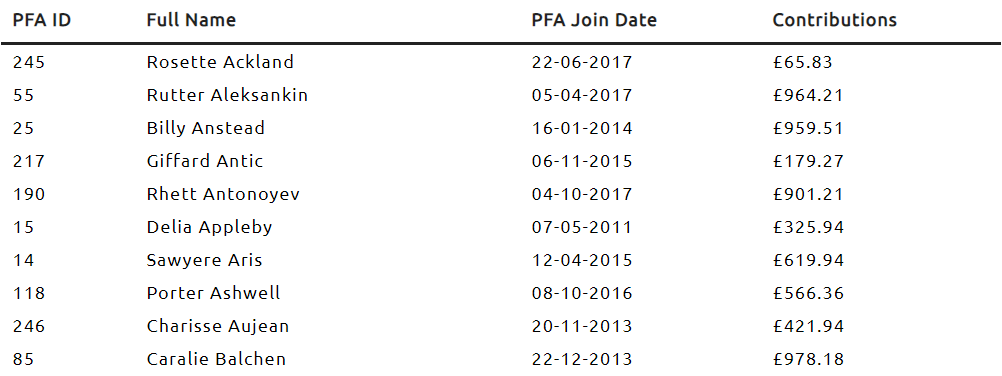
\includegraphics[width=\linewidth]{images/01.png}
\subsection{A List of staff with managers query result}
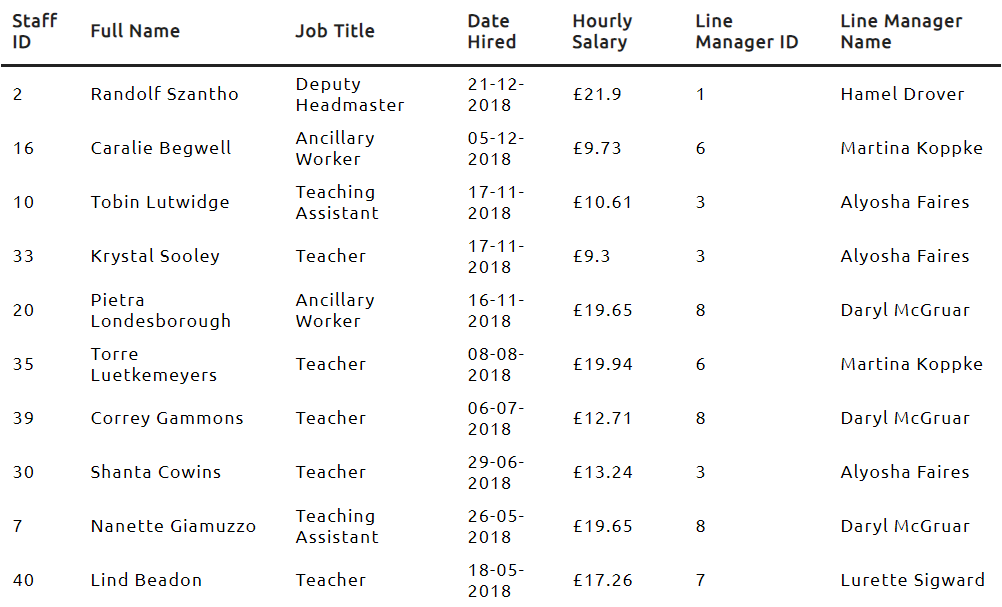
\includegraphics[width=\linewidth]{images/02.png}
\subsection{Resource hire sheet and resource hire booking form}
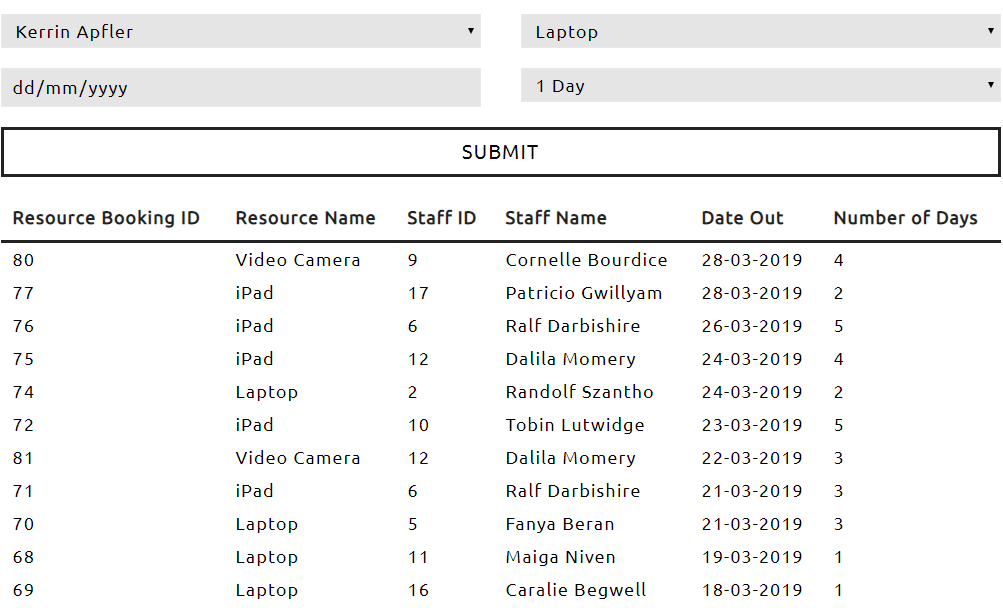
\includegraphics[width=\linewidth]{images/03.png}
\subsection{Faculty teacher listing query result}
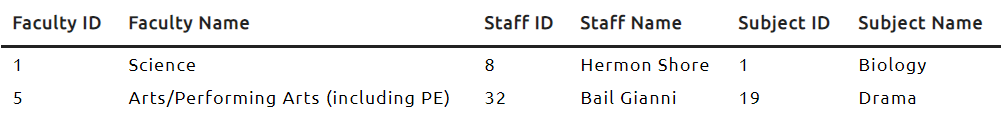
\includegraphics[width=\linewidth]{images/04.png}
\subsection{Faculty member listing query result}
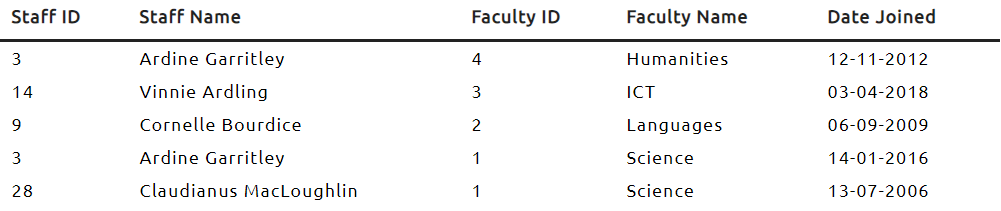
\includegraphics[width=\linewidth]{images/05.png}
\subsection{Room request sheet and booking form}
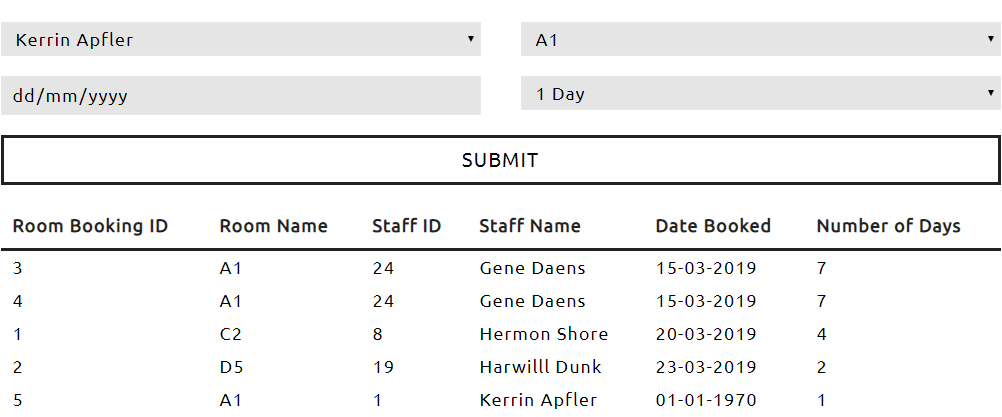
\includegraphics[width=\linewidth]{images/06.png}
\section{Create queries to show each of the following}
\subsection{Teachers who are also parents query result}
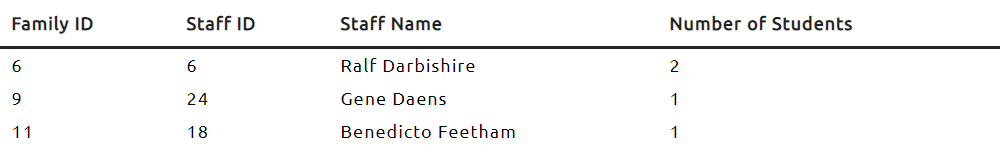
\includegraphics[width=\linewidth]{images/07.png}
\subsection{The resources that have been hired less than 3 times query result}
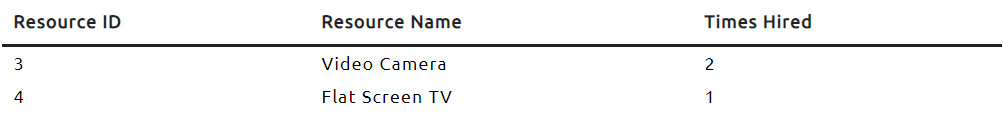
\includegraphics[width=\linewidth]{images/08.png}
\subsection{The staff who have worked for all the departments query result}
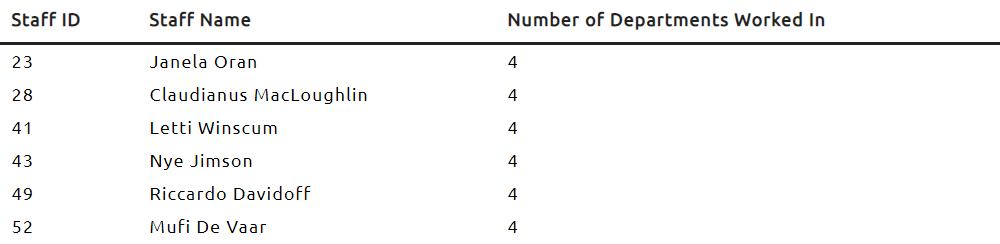
\includegraphics[width=\linewidth]{images/09.png}
\subsection{The details of the teachers, whose surname starts with the same letter as the person who has attended the most meetings query result}
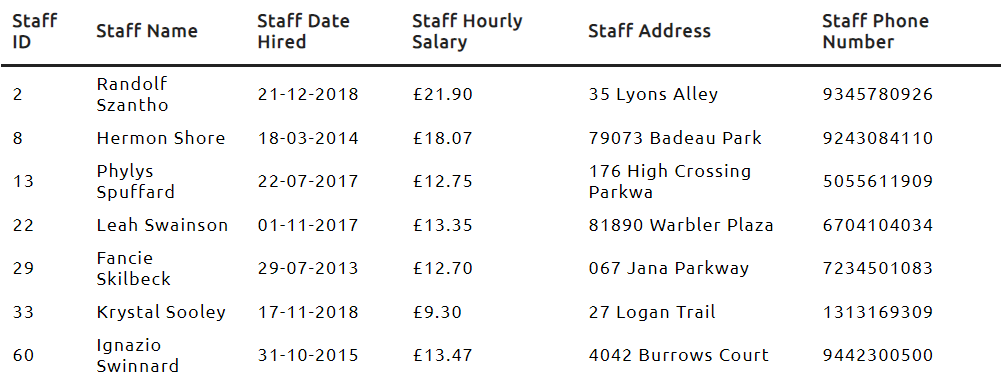
\includegraphics[width=\linewidth]{images/10.png}

\newpage

\printglossary[type=\acronymtype]
 
\printglossary

\lstlistoflistings

\end{document}
